
\chapter{The Vedic Hindu culture and the ancient Tamils: The unity of Hindu civilization}\label{chapter4}

\Authorline{Akshay S. P.}


\section*{Abstract}

Dravidian movement of southern India, especially in the state of Tamil Nadu, needs no detailed introduction. It is based on the notion that the Brahmins and other upper castes are descendants of the Sanskrit speaking Vedic Aryans who invaded from Central Asia and fought off the Dravidians who formerly inhabited the northern regions of India into the southern regions. Even further, the Dravidianists\index{Dravidianists} claim that the Aryan Brahmins also gradually moved into the southern parts of India from northern regions of the country and later enslaved the native Dravidians of south and exploited them by making the native Dravidians follow the `oppressive' Brahmanical Sanskritic Hindu religion and placing them as lower castes. The Dravidianist anti-Sanskrit anti-Brahmanism which has in turn manifested itself into anti-Hinduism is a cause for many attacks on the Hindu traditions and culture in south, directly or indirectly. It is a part of the ‘breaking India’ forces. Many instances of anti-Hindu events have been reported ever since the Dravidian movement gained prominence in south Indian states like Tamil Nadu. Besides this, the Aryan-Dravidian narrations have also crept into the politics of the southern states, causing the north-south divide. This paper aims to refute the claim propagated by the Dravidianists, that the early Dravidians did not adhere to the Vedic Hindu culture, by using textual, archaeological, numismatic\index{numismatic evidences} and epigraphical evidences.\index{epigraphical evidences} Apart from this, the paper also tries to establish that there was a notion of unified Dhārmic civilization among the inhabitants of early historic Indian subcontinent without any north-south cultural distinction. Since the Dravidian movement more or less revolves around the Tamils and since Tamil is the oldest properly recorded Dravidian language with a vast literature and several early inscriptions (as all other early historic inscriptions from the modern Dravidian speaking regions like in the Deccan are in Prakrit\index{Prakrit} languages), this paper gives emphasis on the early Tamil culture and traces its Vedic elements.


\section*{Introduction}

One of the major accusation of the members who started the Dravidian movement\index{Dravidian movement} was that ‘Aryan’ Brahmins who are descendants of the ancient Sanskrit speaking Vedic Aryan intruders openly exploited the native Dravidians, and that the ancient Dravidians were not followers of the Vedic Hindu religion and had their own separate native culture which was later destroyed or appropriated by the incoming Aryan intruders. Many authors have even claimed that the bronze-age Harappan civilization\index{Harappan civilization} was the original civilization of the Dravidians which was destroyed or assimilated during later periods by incoming Aryan hordes. Hence, these authors have tried to trace and reconstruct glorious pre-Vedic Aryan or non-Hindu past of the Dravidians, especially of the early Tamils.

The earliest recorded Tamil history as we know is from the period known as the Caṅkam age.\index{Cankam age@Caṅkam age} This period lasted from around 500-300 BCE to around 300 CE. Most of the information about this period is gained from sources like coins, inscriptions, texts composed during this period etc. The Cēra,\index{Cera@Cēra} the Cōḻa\index{Cola@Cōḻa} and the Pāṇdya\index{Pandya@Pāṇdya} were three of the most powerful kingdoms of ancient Caṅkam age Tamil lands which constituted modern southern Indian states of Kerala and Tamil Nadu. Mauryan emperor Ashoka\index{Ashoka} mentions these kingdoms as his southern neighbours in his edicts during third century BCE. Caṅkam age literature includes poetic works like Puṟanāṉuṟu,\index{Purananuru@Puṟanāṉuṟu} Akanāṉūṟu,\index{Akananuru@Akanāṉūṟu} Paripāṭal,\index{Paripatal@Paripāṭal} Kalittokai, Aiṅkuṟunūṟu, Patiṟṟuppattu, Kuṟuntokai etc.

If one goes through the early Tamil literature along with other sources like numismatics, archaeology etc, one will find that there is no reason to imagine a distant pre-Vedic past of the Tamil culture and that the Vedic and even the post Vedic culture was firmly established in ancient Tamil lands since earliest recorded period. It is also to be mentioned that Buddhism and Jainism were also present in ancient Tamil lands, but to detail about them is beyond the scope of this paper as it specifically deals with Vedic and post-Vedic Hindu elements in ancient Tamil kingdoms.


\section*{Vedic Hinduism in ancient Caṅkam age\index{Cankam age@Caṅkam age} Tamil lands:}

Contrary to the Dravidianist claims that early Tamils did not follow Vedic religion, if one goes through the early Caṅkam age Tamil texts without any bias, one can easily understand that the early Caṅkam age Tamil kings were staunch followers of ancient Vedic religion.

For example an early Pāṇdyaṉ king named Palyākacālai Mutukuṭumi Peruvaḻuti\index{Peruvaluti@Peruvaḻuti} who is mentioned in Puṟanāṉuṟu\index{Purananuru@Puṟanāṉuṟu} held the Sanskritic title ‘Palyākacālai’\index{Palyakacalai@Palyākacālai} since he built many sacrificial halls and performed Vedic rituals as narrated in from Puṟanāṉuṟu poem 15.

\begin{myquote}
“Given your rage, which one of these is greater in number – the eager enemy foot soldiers who retreated in shame and live with blame, after they came with a desire to ruin your strength, brandishing their tall spears that throw shadows and beautiful shields made with iron, to fight against your army with shining weapons, or the number of huge fields where you have planted columns after performing faultless rituals prescribed by the four good Vedas, with precious sacrificial elements and abundant ghee?”\hfill (Puṟanāṉuṟu 15 Translation by Vaidehi Herbert.) 
\end{myquote}

Here the term \textit{āvuti} which is derived from Sanskrit \textit{āhuti}\index{ahuti@\textit{āhuti}} or offerings made in sacred sacrificial fire is mentioned.

\vskip 5pt

In fact the Caṅkam age Pāṇdyaṉ kings had issued coins depicting the theme of Vedic sacrifice, with animals tied to the sacrificial posts. Some Pāṇdyaṉ coins depict image of a horse tied to a standard (Figure~\ref{art5-fig1}) which could be a Vedic sacrificial standard named \textit{yūpa.}\index{yupa@\textit{yūpa}} There is also a circle and a crescent or half circle symbols near to it. These symbols may represent Vedic \textit{gārhapatya}\index{garhapatya@\textit{gārhapatya}} and \textit{dakṣiṇāgni}\index{daksinagni@\textit{dakṣiṇāgni}} altars respectively. This depiction could indicate the performance of Vedic \textit{Aśvamēdha}\index{Asvamedha@\textit{Aśvamēdha}} or horse sacrifice performed by powerful Vedic monarchs.

\begin{figure}[!htbp]
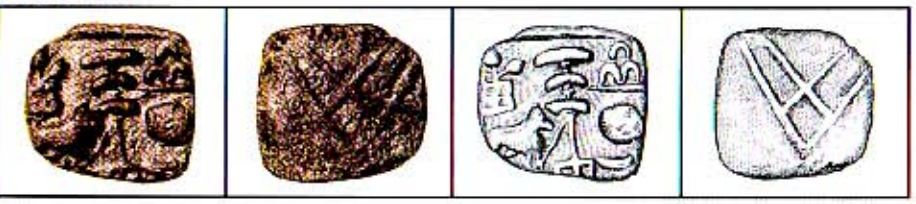
\includegraphics{"images/article-05/art05-fig01.jpg"}
\caption{A Caṅkam age Pāṇdya coin depicting a horse tied to a standard. Courtesy of Krishnamurthy \& Wickramasinghe 2005: 29, Coin No.13.}\label{art5-fig1}
\end{figure}

The triple-umbrella shaped standard in the Pāṇdyaṉ\index{Pandya@Pāṇdya} coin to which the horse is tied can also be noticed in coins of the Pāñcāla kingdom (Figure~\ref{art5-fig2}) which are dated to the early historic period, contemporary to the Caṅkam age. Pāñcāla kingdom was part of the larger Kuru-Pāñcāla realm which was considered as the stronghold of Vedic culture since the ancient Vedic period.

\begin{figure}[!htbp]
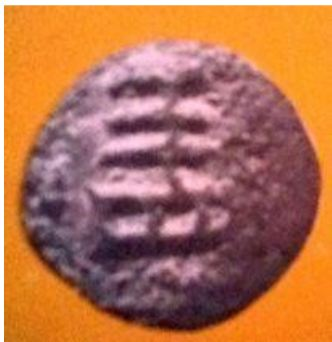
\includegraphics{"images/article-05/art05-fig02.jpg"}
\caption{ A Pāñcāla coin depicting a triple-umbrella shaped standard. Courtesy of Shrimali 1985: Plate XI. Coin 8.}\label{art5-fig2}
\end{figure}

So this is a clear evidence for the practice of ancient Vedic sacrifices in early Caṅkam age Pāṇdyaṉ kingdom.

Apart from Pāṇdyaṉ Peruvaḻuti, a Cōḻa\index{Cola@Cōḻa} king named Irācacūyam\index{Iracacuyam@Irācacūyam} Vēṭṭa Perunaṟkiḷḷi\index{Vetta Perunarkilli@Vēṭṭa Perunaṟkiḷḷi} is praised in poems from Puṟanāṉuṟu 16, 367, 377 etc. He held the Sanskritic title ‘Irācacūyam Vēṭṭa’ for performing the Vedic \textit{Rājasūya}\index{Rajasuya@\textit{Rājasūya}} ritual which was performed by the most powerful Vedic kings.

Another Cōḻa\index{Cola@Cōḻa} king named Karikālaṉ\index{Karikalan@Karikālaṉ} is said to performed Veda vēḷvi or Vedic sacrifices in Puṟanāṉūṟu\index{Purananuru@Puṟanāṉūṟu} 224.

\begin{myquote}
“Surrounded by his faultless women with pure principles, he performed Vedic rituals in the court of righteousness where justice is practiced, where those with knowledge stand and praise, within the many circular walls where a post rises next to where vultures are fed.”

~\hfill (Puṟanāṉūṟu 224 translated by Vaidehi Herbert.)
\end{myquote}

Also, many Cōḻa rulers held the title Cempiyaṉ.\index{Cempiyan@Cempiyaṉ} This title in fact is derived from the Sanskrit patronym Śaibya, meaning descendants of the benevolent Vedic king Śibi who's story is famous among Hindus (there's also a Buddhist Jataka\index{Buddhist Jataka} narrating his story). The story of king Śibi is mentioned at various places in the Caṅkam literature, like Puṟanāṉūṟu 37, 46 etc. The early Cōḻa kings claimed origins from the northern king by keeping the title Cempiyaṉ.

Apart from Cōḻa and Pāṇdyaṉ kings, the Cēra\index{Cera@Cēra} kings were also followers of the Vedic culture.

Patiṟṟuppattu\index{Patirruppattu@Patiṟṟuppattu} 21 also mentions a Cēra king named Palyāṉai Celkeḻu Kuṭṭuvaṉ\index{Palyanai Celkelu Kuttuvan@Palyāṉai Celkeḻu Kuṭṭuvaṉ} performing Vedic rites with oblations into the fire (āvuti or āhuti).

\begin{myquote}
“These esteemed sages are noble, truthful and dependable like the morning sun. They worship gods and perform rituals according to their strong traditions. The bright flames they light for oblations that yield benefits, are like reflections of their inner desires. Smoke rises from their ritual fires.”\hfill (Patiṟṟuppattu 21 translated by Vaidehi Herbert.)
\end{myquote}

So these poems are testimony for the fact that the kings from all three of the greatest Tamil kingdoms performed Vedic rituals during Caṅkam age.

Further, Puṟanāṉuṟu 166 praises a Vedic Brahmin named Kauṇiyaṉ\index{Kauniyan@Kauṇiyaṉ} (Kauṇḍinya in Sanskrit) Viṇṇantāyaṉ\index{Vinnantayan@Viṇṇantāyaṉ} as a heir of Vedic ritualists who had performed all 21 Vedic \textit{yajña}-s (7 \textit{soma, havir} and \textit{pāka yajña}-s) and engaged in Vedic debates.

\begin{myquote}
“You who is an heir of learned men who performed the twenty-one rituals without fault, who understood those who disrespected and spoke truth-like lies, defeating those who would contend with the ancient work of four divisions and six sections, focused on righteousness, never swerving from the well chosen words of the ancient Being with long matted hair.”\hfill (Puṟanāṉuṟu 166 Translation by Vaidehi Herbert.)
\end{myquote}

There are also references to the three sacred fires or muttī (\textit{trētāgni}\index{tretagni@\textit{trētāgni}} in Sanskrit), i.e \textit{gārhapatya},\index{garhapatya@\textit{gārhapatya}} \textit{dakṣiṇāgni\index{daksinagni@\textit{dakṣiṇāgni}} and āhavanīya} fires maintained by Vedic ritualists, in Puṟanāṉūṟu 2 \& 367.

\begin{myquote}
“Even if milk turns sour, the sun darkens, or the four Vedas swerve from the truth, may you totally glow, with your unswerving ministers! May you never be shaken like Mount Pothiyam, like the Himalayas with its golden summits, where long-eyed does sleep on the slopes near their fawns with tiny heads, at dusk, in the light of three fires lit by the brahmins who perform difficult rituals!”

~\hfill (Puṟanāṉūṟu 2 translated by Vaidehi Herbert.)
\end{myquote}

\begin{myquote}
“You kings who ride in chariots with flags and own victorious white umbrellas, beautiful to behold like the three flames of the twice-born brahmins who have subdued their senses through their will! This is what I understand!  May your living days be splendid!  May they be brighter than the stars in the sky!  May they be more than the raindrops from the dark thundering clouds!”

~\hfill (Puṟanāṉūṟu 367 translated by Vaidehi Herbert.)
\end{myquote}

Apart from Vedic rituals, an old Tamil poem from Aiṅkuṟunūṟu\index{Ainkurunuru@Aiṅkuṟunūṟu} 62 mentions a Vedic festival dedicated to Vedic God Indra:\index{Indra}

\begin{myquote}
“Lord!  You attract women in this town, where a peahen, with its tiny head looking like the flowers of Inthira festival, calls her mate from a strip of shade. Which town will your chariot stop next?”

~\hfill (Aiṅkuṟunūṟu 62 Translated by Vaidehi Herbert.)
\end{myquote}

Further, Tolkāppiyam,\index{Tolkappiyam@Tolkāppiyam} the oldest Tamil grammatical work also mentions Vedic God Varuna by his Sanskrit name as the deity of coastlands and the name of the text \textit{kāppiyam} itself is derived from Sanskrit term \textit{kāvya}. In later tradition, Tolkāppiyar\index{Tolkappiyar@Tolkāppiyar} who is the author of Tolkāppiyam became regarded as a student of sage Agastya\index{Agastya} who is said to have received the Tamil language from God Śiva and the first Vedic sage to settle down in southern India.

Also, it is to be noted that many of the Caṅkam age\index{Cankam age@Caṅkam age} authors were Brahmins and had Vedic Sanskrit names like Gautama (Akanāṉuṟu 159, Patiṟṟuppattu 21-30), Kauśika (Puṟanāṉūṟu\index{Purananuru@Puṟanāṉūṟu} 309, Akanāṉuṟu\index{Akananuru@Akanāṉuṟu} 66, 381 etc) Kapila etc. Among these, an author named Kapilar\index{Kapilar} was the most famous one and he had contributed a lot to the Caṅkam literature. In fact Kapilar took care of the daughters of a chieftain named Vēl Pāri\index{Vel Pari@Vēl Pāri} as narrated in Puranānūru 201 after he was killed in battle. So the Vedic Brahmins were viewed as trustworthy people with high esteem by the ancient Tamil society.

Further Puṟanāṉūṟu 9 specifically gives warning to Brahmins, cows, women, disabled people etc to evacuate the town as the battle is about to start.

\begin{myquote}
“Cows, Brahmins with the nature of cows, women, those who are sick, and those living in the Southern Land with no gold-like sons to perform precious last rites, take refuge!   We are ready to shoot volleys of arrows!”\hfill (Puṟanāṉūṟu 9 Translated by Vaidehi Herbert.)
\end{myquote}

Similarly when Kaṇṇaki,\index{Kannaki@Kaṇṇaki} the heroine of the famous Tamil epic Cilappatikāram\index{Cilappatikaram@Cilappatikāram} was about to burn the city of Madurai out of her wrath, she asked fire God Agni to spare Brahmins, cows, women etc. This would indicate that the Brahmins and cows were viewed respectfully by the society and the notion of \textit{Brahmahatyā}\index{Brahmahatya@\textit{Brahmahatyā}} and \textit{Gōhatyā}\index{Gohatya@\textit{Gōhatyā}} or the sins of killing Brahmins and cows were popular among Caṅkam age\index{Cankam age@Caṅkam age} Tamils. Even until around 17th-18th centuries in Kerala, these concepts survived, and warriors and kings had to take oaths to protect Brahmins and cows. Thus the notion of \textit{Brahmahatyā} and \textit{Gōhatyā} in southern India goes way back to the Caṅkam age more than 2000 years ago.

All these evidences from early Caṅkam age Tamil literature proves that the Vedic ‘Brahmanism’ or the worship of Vedic Gods and rituals along with Sanskrit speaking Brahmins were firmly established in Tamil lands during early Caṅkam era.


\section*{Post-Vedic Hinduism in ancient Caṅkam age Tamil lands:}

Apart from the ancient Vedic Hinduism, the Āgama-Tāntric\index{Agama-Tantric@Āgama-Tāntric} (i.e the post Vedic Hinduism where temple and image worship became popular) or Itihāsa-Purānic\index{Itihasa-Puranic@Itihāsa-Purānic} form of Hinduism was also practiced in Caṅkam age Tamil kingdoms. Puṟanāṉuṟu poem 6 describes Pāṇdyaṉ king Peruvaḻuti\index{Peruvaluti@Peruvaḻuti} visiting temple of three eyed God i.e Śiva, and the poem also praises the king by saying he only bows his head down in front of Vedic Brahmins to get their blessings.

\begin{myquote}
“May your umbrella bow down only when it circumambulates the temple of the god with three eyes! May your head bend down only when the brahmins of four Vedas lift their hands!”

~\hfill (Puṟanāṉuṟu 6 Translation by Vaidehi Herbet.)
\end{myquote}

Śiva\index{Siva@Śiva} is claimed by many as a non-Aryan Dravidian God appropriated by Aryans. But if we go through the early numismatic evidences,\index{numismatic evidences} it is not only apparent that the early Tamils widely worshiped Śiva, but it also makes it clear that the Śiva worship in Tamil lands came from northern India.

For example Caṅkam age coins of Pāṇdyaṉ (Figure~\ref{art5-fig3}) and Cēra (Figure~\ref{art5-fig4}) kingdoms depicts an elephant standing in front of a trident shaped standard with an axe attached to it on the side. The Pāṇdyaṉ\index{Pandya@Pāṇdya} coin also depicts a human figure nearby (possibly Śiva himself).

\begin{figure}[H]
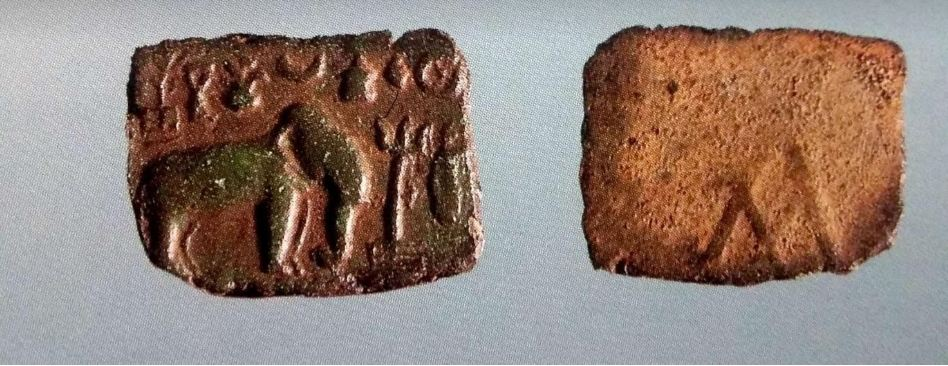
\includegraphics[scale=1.1]{"images/article-05/art05-fig03.jpg"}
\caption{Caṅkam age Pāṇdyaṉ coin with elephant in front of a trident-axe standard along with a human figure and Pāṇdyaṉ royal insignia fish symbol on reverse. Courtesy of Krishnamurthy 1997: Plate 4, coin~52.}\label{art5-fig3}
\end{figure}


\begin{figure}[H]
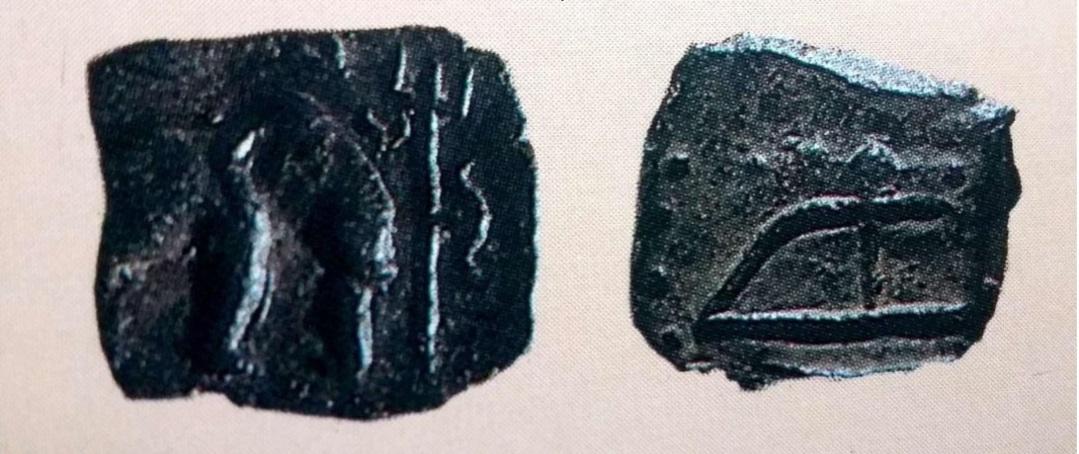
\includegraphics{"images/article-05/art05-fig04.jpg"}
\caption{Caṅkam age Cēra coin with elephant in front of a trident-axe standard and Cēra royal insignia bow \& arrow symbol on reverse. Courtesy of Krishnamurthy 1997: Plate 10, coin 119.}\label{art5-fig4}
\end{figure}

This triśūla\index{trisula@triśūla} or trident\index{trident} with axe symbol was an early symbol associated with God Śiva. The same symbol can be seen in northern coins of same period as well, for example we can see it in the coins of northern Indian Vemaka tribe\index{Vemaka tribe} from near Himalayas (Figure~\ref{art5-fig5})

\begin{figure}[!htbp]
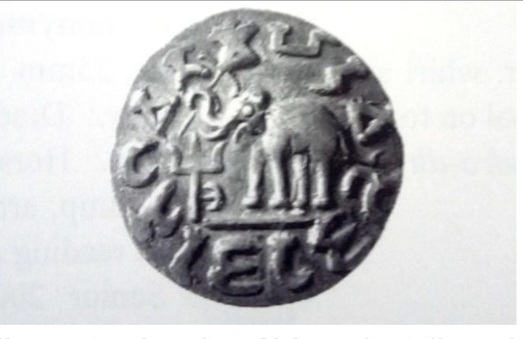
\includegraphics{"images/article-05/art05-fig05.jpg"}
\caption{A coin of Vemaka tribe with elephant standing in front a trident-axe standard. Courtesy of Pieper 2013: Page 383, coin 1148.}\label{art5-fig5}
\end{figure}

Also the coins of Kuninda tribe\index{Kuninda tribe} from the same era which inhabited regions close to Himalayas also depicts Śiva\index{Siva@Śiva} holding trident-axe\index{trident} weapon (Figure~\ref{art5-fig6})

\begin{figure}[!htbp]
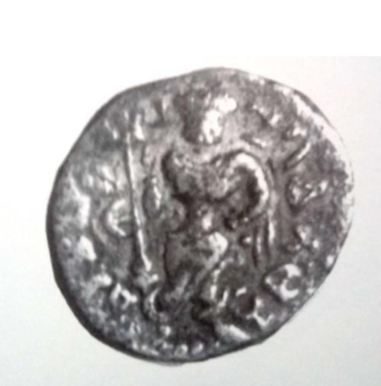
\includegraphics{"images/article-05/art05-fig06.jpg"}
\caption{Kuninda coin depicting Śiva holding triśūla with axe attached to it. Courtesy of Handa 2007: Plate LXXIX.}\label{art5-fig6}
\end{figure}

Further, coins of Audumbara tribe\index{Audumbara tribe} from Punjab dated to same era frequently depicts the same trident-axe\index{trident} standards in front of temples which were obviously dedicated to Śiva (Figure~\ref{art5-fig7}).

\begin{figure}[!htbp]
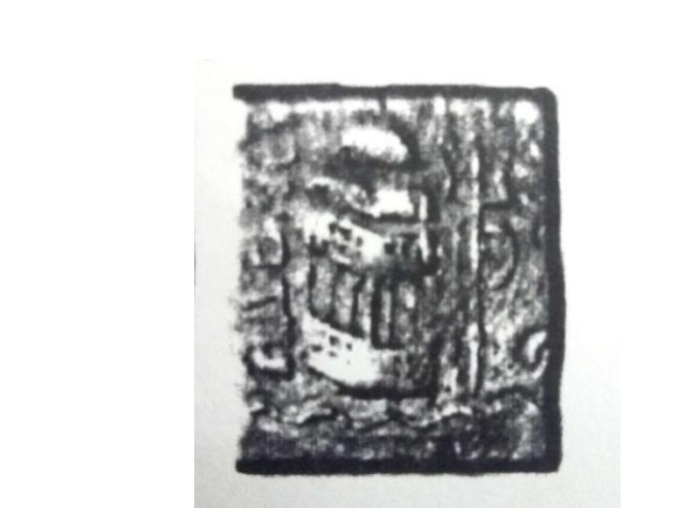
\includegraphics{"images/article-05/art05-fig07.jpg"}
\caption{Coin of Audumbara tribe depicting a temple with trident-axe standard in front. Courtesy of Handa 2007:\break Plate VI, coin 3.}\label{art5-fig7}
\end{figure}

So we can trace the origins of the trident-axe weapon standard, which was a symbol representing God Śiva, from far northern India all the way into the southern Tamil lands during the early historic period. Thus the early Śiva worship spread from northern regions into the southern parts.

It is also to be noted that many people still view Murukaṉ\index{Murukan@Murukaṉ} (Skanda\index{Skanda} or Kārtikēya in Sanskrit tradition) who is the son of Śiva as a native Dravidian God. It is true that Murukaṉ is known as the most adored God among Tamils. But it is also an undeniable fact that even the early worship of Murukaṉ had origins in northern regions. The earliest ever depictions of Murukaṉ or Skanda is found in art from northern regions. There are numerous early depictions of Murukaṉ\index{Murukan@Murukaṉ} or Skanda\index{Skanda} from ancient early historic sites of northern India like Mathura, like the one (Figure~\ref{art5-fig8}) shown as an example here.

\begin{figure}[!tb]
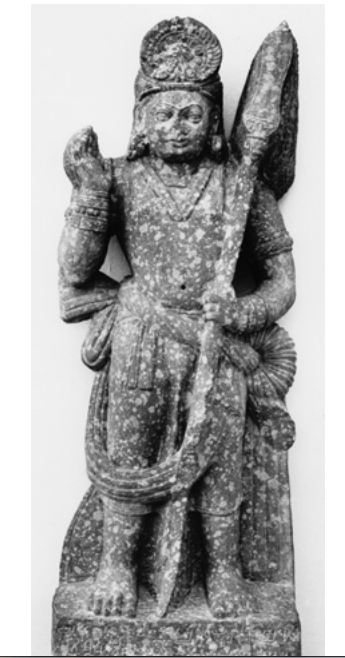
\includegraphics{"images/article-05/art05-fig08.jpg"}
\caption{Early depiction of Murukaṉ\index{Murukan@Murukaṉ} with his trademark weapon vēl or spear from Mathura, dated to early CE. Courtesy of Mann 2011: 265, Figure 15. (Courtesy of the American Institute for Indian Studies and the Mathura Government Museum).}\label{art5-fig8}
\end{figure}

Murukaṉ is also depicted in various coins from northern India during early historic period, like in the coins of Yaudheya tribe\index{Yaudheya tribe} from Punjab (Figure~\ref{art5-fig9})

\begin{figure}[!tb]
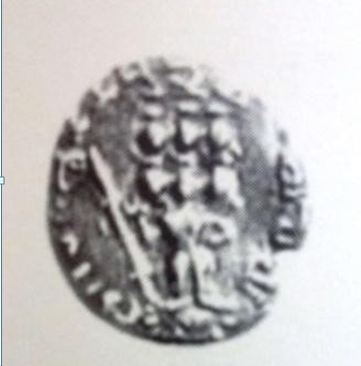
\includegraphics{"images/article-05/art05-fig09.jpg"}
\caption{Coin of Yaudheya tribe depicting Murukaṉ with six heads and holding vēl. Courtesy of Handa 2007: Plate XLII.}\label{art5-fig9}
\end{figure}

At the same time during the Caṅkam age\index{Cankam age@Caṅkam age} in Tamil lands, there are no popular depictions of Murukaṉ like we have in northern India.

It is also to be noted that Caṅkam age text named Paripāṭal\index{Paripatal@Paripāṭal} which contains popular Hindu Puranic narrations\index{Puranic narrations} also states that the birth of Murukaṉ took place in northern Himalayas.

\begin{myquote}
“The embryo was hacked to pieces. The seven sages who understood this to be the future commander of the Celestials, received them. Thinking that their chaste wives would not agree to carry them in their wombs to fullness, they threw them into the sacrificial fire pit. The triple-fire fostered them and left them purified. Among the seven women flourishing in the north, barring chaste Arunthathi, the other six, wives of great sages, without losing their chastity, carried in their wombs the embryo. In the lofty Himalayas, in a spring with blue waterlilies, you were born in the center of a lotus, O Lord!” 

~\hfill (Paripāṭal translation by Vaidehi Herbert.)
\end{myquote}

So clearly, the worship of Murukaṉ also came from north in early historic periods into Tamil lands.

While mentioning Itihasa-Puranic themes, it is also to be mentioned that the epic Rāmāyaṇa\index{Ramayana@Rāmāyaṇa} is one of the most hated text by the Dravidianists since according to them it speaks of the conquest of southern India by ‘Aryan’ Rāma\index{Rama@Rāma} from north. But Caṅkam era poems like Akanāṉūṟu\index{Akananuru@Akanāṉūṟu} 70 \& Puṟanāṉuṟu\index{Purananuru@Puṟanāṉuṟu} 378 already mention Rāmāyaṇa\index{Ramayana@Rāmāyaṇa} theme without any such hostility:

\begin{myquote}
“Now, the wedding has been arranged, and gossip has died down in this loud town, like the sounds of birds on banyan trees with aerial roots, which died down when Raman who wins wars was planning strategies, in the ancient, roaring Kōdikarai port town belonging to the Pāndiyan king, where golden \textit{gnālal} and \textit{punnai} blossoms decorate the groves near the lovely, big port, and women decorate themselves for festivals with garments made with  waterlilies that flourish in abundance with thick stems and beautiful, huge leaves.”

~\hfill (Akanāṉūṟu 70 translated by Vaidehi Herbert.)
\end{myquote}

\begin{myquote}
“They were like a huge family of monkeys with gaping red mouths scooping up the beautiful ornaments that fell to the ground, when the mighty demon snatched away enraged Raman’s wife Seethai.  Heading a large family and thinking about removing their great sorrow, I was very happy along with them when our poverty and distress were removed.”

~\hfill (Puṟanāṉuṟu 378 translated by Vaidehi Herbert.)
\end{myquote}

Thus, it is easily understandable that Rāmāyaṇa\index{Ramayana@Rāmāyaṇa} themes were popular among Caṅkam age Tamils. This totally contradicts the claim of the leaders of Dravidian movement that Rāmāyaṇa was alien to early Tamils and establishes the fact that ancient Tamils praised and worshiped the valour of Rāma.\index{Rama@Rāma}

Apart from Rāmāyaṇa, themes from Mahābhārata can also be found in Caṅkam\index{Cankam@Caṅkam} age texts. For example Puṟanāṉuṟu 2 mentions Cēra\index{Cera@Cēra} king Utiyaṉ Cēralātaṉ\index{Ceralatan@Cēralātaṉ} feeding the armies of the five and the hundred i.e Pāṇḍava\index{Pandava@Pāṇḍava} and Kaurava\index{Kaurava} armies in the Kurukṣētra battle.\index{Kuruksetra battle@Kurukṣētra battle}

\begin{myquote}
“You are king of a country with prosperous towns!  The sky is your limit! O Greatness who gave unlimited food, until those hundred men wearing golden \textit{thumpai} flower garlands had seized the land and perished in the field fighting furiously against the five whose horses wore swaying plumes!”\hfill (Puṟanāṉuṟu 2 translated by Vaidehi Herbert.)
\end{myquote}

So clearly, if we look into the Caṅkam Tamil literature we can understand that both the Vedic and the post Vedic Hindu elements were popular among the ancient Tamil society.


\section*{Archaeological and numismatic evidences for Vedic elements during early Caṅkam age:}

There are also conclusive archaeological evidences for the fact that Vedic and post Vedic Hindu elements had strong presence in Tamil lands during Caṅkam\index{Cankam@Caṅkam} age. In fact from archaeological evidences it is clear that the Tamils had contact with northern cultures and also adopted material culture of north. As noted archaeologist Dilip K. Chakrabarti\index{Chakrabarti, Dilip K.} writes:

\begin{myquote}
“Period I of Alagukalam\index{Alagukalam} has red ware, black-and-red ware, mat-design pottery, NBP and grey ware and its dominant pottery is black and red ware. There is no radio carbon date from the level, and the excavators’ chronology puts it between 500 BC and 300 BC. I think that there is enough justification to put it between the bracket 700/800 BCE to 400 BCE. The NBP occurs in the upper level and may be put anywhere between 500 and 400 BCE.”\hfill (Chakrabarti 2008:109)
\end{myquote}

This NBP or the Northern Black Polished Ware (NBPW)\index{Northern Black Polished Ware (NBPW)} culture was the material culture of northern janapada states of the post Vedic period. The presence of NBPW in Tamil lands during early Caṅkam age, i.e 500-400 BCE, indicates that Tamils back then had adopted same culture as the northern Janapada states. Black and red ware or BRW\index{Black and red ware or BRW} culture was also found in northern regions during the Iron age. Also the early Caṅkam age Pāṇdyans\index{Pandya@Pāṇdya} had issued punch-marked coins (Figure~\ref{art5-fig10}) which were associated with the northern janapada states.

\begin{figure}[!htbp]
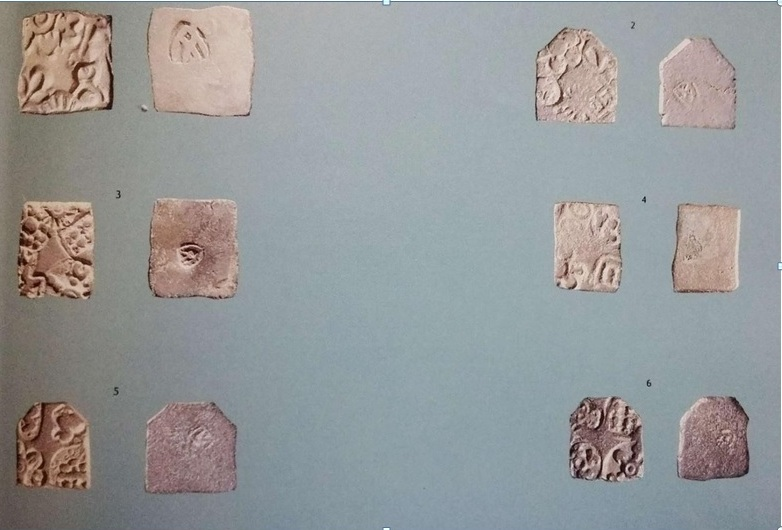
\includegraphics{"images/article-05/art05-fig10.jpg"}
\caption{The early Caṅkam age punch-marked coins of Pāṇdyan kingdom. Photo courtesy of Krishnamurthy 1997: Plate 1, coins 1-6.}\label{art5-fig10}
\end{figure}

Further, many early southern coins of Tamil kingdoms have typical Dhārmic symbols like \textit{svastika},\index{svastika} \textit{śrīvatsa},\index{srivatsa@śrīvatsa} \textit{nandipada},\index{nandipada} tree shrines, hill shrines etc along with other symbols found in the art and coins of the northern \textit{janapada} states. This indicates that the proper urbanism, statehood, trade and the currency system was adopted from northern regions by the ancient Tamils. Before these were adopted, southern regions were in non-urban megalithic era.

Also apart from this, it is highly possible that the Caṅkam age Tamils also followed the same architectural style as seen in northern regions of early historic period India. For example a Caṅkam age coin (Figure~\ref{art5-fig11}) of the Pāṇdyan kingdom depicts a temple which uses the architectural style with arches as we can see in early northern buildings depicted in art and carvings from sites like Ajanta,\index{Ajanta} Karla caves\index{Karla caves} etc.

\begin{figure}[!htbp]
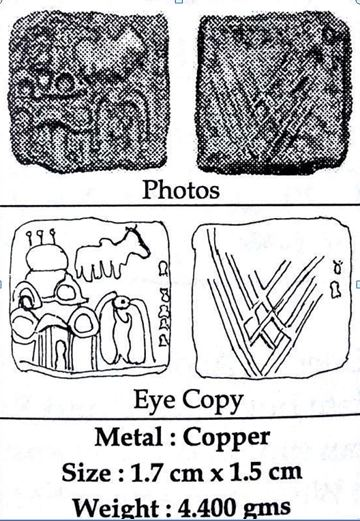
\includegraphics{"images/article-05/art05-fig11.jpg"}
\caption{Caṅkam age coin of Pāṇdyan kingdom kingdom depicting a building, which is most likely an ancient temple, along with bull and a pond, Pāṇdyaṉ royal insignia fish symbol on reverse side. Photo courtesy of Krishnamurthy 2016: Page 272.}\label{art5-fig11}
\end{figure}

This architectural style using particular style of arches continued to be used in later Pallava\index{Pallava} and even later Cōḻa\index{Cola@Cōḻa} architecture, which means that the even the widely known ‘Dravidian’ architecture\index{Dravidian architecture} has it’s roots in Caṅkam age architecture which in turn has it’s origins in northern regions.

Also, the Tamils in early period used the Brahmi\index{Brahmi} writing system, same as in northern region. Many Tamil Brahmi inscriptions from Tamil lands also shows borrowings from northern Prakrit languages as well. This means Prakrit\index{Prakrit} and obviously Sanskrit was also known in ancient Caṅkam\index{Cankam@Caṅkam} age Tamil regions.


\section*{Unity of North and South India under same civilization during early historic period:}

Caṅkam age Tamil poems like Puṟanāṉuṟu 132 treat the lands from Himalayas\index{Himalayas} to southern lands as one entity.

\begin{myquote}
“In the North, on the sky-high Himalayas, a deer eats oranges and grazes on \textit{naranthai} grass, drinks water from a spring with kuvalai flowers and rests with its mate in the shade of a cool \textit{thakaram} tree. If it were not for the lineage of Ārya in the South, this wide world would turn upside down!”

~\hfill (Puṟanāṉuṟu 132 translation by Vaidehi Herbert.)
\end{myquote}

It is to be noted that the Kaliṅga\index{Kalinga@Kaliṅga} king Kharavela\index{Kharavela} who ruled during 2nd century BCE speaks of conquering Tamil kingdoms when he started the conquest of the kingdoms within Bhāratavarṣa or Indian subcontinent in his Hathigumpha inscription.\index{Hathigumpha inscription} This indicates that the early Tamil kingdoms were part of Bhāratavarṣa civilization of south Asia and there was a common civilizational identity.

Further an epilogue from Patiṟṟuppattu\index{Patirruppattu@Patiṟṟuppattu} makes mention of the Cēra king Cēraṉ Ceṅkuṭṭuvaṉ\index{Ceran Cenkuttuvan@Cēraṉ Ceṅkuṭṭuvaṉ} washing the idol of Goddess Kaṇṇaki\index{Kannaki@Kaṇṇaki} or Pattiṉi in the sacred waters of Gaṅga river in north. This clearly proves that the Caṅkam age Tamils back then viewed the Gaṅga river as a sacred river just like the modern Hindus do.

\begin{myquote}
“He defeated a noble Aryan king of great renown, to get a stone to make Pathini Goddess a statue, going rapidly like an arrow going through a windy forest, washed it in the Ganges whose waters come from many sweet waterfalls, and seized and brought many fine breeds of cattle herds with calves.”

~\hfill (An epilogue from Patiṟṟuppattu translation by Vaidehi Herbert.)
\end{myquote}

Kaṇṇaki\index{Kannaki@Kaṇṇaki} or Pattiṉi was the heroine of the famous Tamil epic Cilappatikāram\index{Cilappatikaram@Cilappatikāram} which was probably composed during later part of the Caṅkam age. She was deified into a Goddess and her worship survives to this day among Tamil Hindus.

Also, Cēraṉ Ceṅkuṭṭuvaṉ\index{Ceran Cenkuttuvan@Cēraṉ Ceṅkuṭṭuvaṉ} defeating Aryan kings in the above passage from Patiṟṟuppattu should not be taken as a sign of war or battle between Aryans and Dravidians. In the Caṅkam Tamil texts the term Aryan or \textit{āriyar}\index{ariya@āriya} is simply used to denote the northerners. In fact Caṅkam age Tamil poem from Kuṟuntokai\index{Kuruntokai@Kuṟuntokai} 184 was composed by a northern Aryan king named Brahmadatta\index{Brahmadatta} who learned Tamil! So, the clash with \textit{āriyar} should only be viewed as clash between northern kingdoms within same civilization to which the Tamil kingdoms were also part of.

All these evidences show that the unity of north and south India under same Dhārmic civilization existed at least for last 2500 years. Since the earliest recorded culture of the Tamils was already under Dhārmic influence, we can say that Tamils were Dhārmic Hindus since time immemorial and that there are no civilizational divides between the Aryans and early Dravidians in recorded history. Tamils having their own terms for Vedic elements like \textit{Pārppaṉar}\index{Parppanar@\textit{Pārppaṉar}} or \textit{Antaṇar}\index{Antanar@\textit{Antaṇar}} (Brahmins) \textit{pūṇūl}\index{punul@\textit{pūṇūl}} (sacred thread), \textit{vēḷvi}\index{velvi@\textit{vēḷvi}} (\textit{yajña}), nāṉmaṟai\index{nanmarai@nāṉmaṟai} (Veda-s) and also names of deities like Koṟṟavai\index{Korravai@Koṟṟavai} (Durga or Kālī), Māyōṉ\index{Mayon@Māyōṉ} \& Tirumāl\index{Tirumal@Tirumāl} (Krṣṇa or Viṣṇu), Vāliyōṉ\index{Valiyon@Vāliyōṉ} (Bālarāma) etc proves that the ancient Tamils viewed Vedic Hindu culture as their own.


\section*{Conclusion:}

Since it is now established that the earliest attested Caṅkam age Tamils were already practicing the Vedic and post Vedic forms of Hinduism, there is no need for a separate Dravidian cultural identity and there is also no need to speculate about an imaginary oppression by Vedic Aryan intruders during pre-historic times of which we have no evidence or records of.

Instead of any sudden violent spread, the Vedic Hindu culture all likely spread from the Vedic \textit{Āryāvarta} region\index{Aryavarta region@\textit{Āryāvarta} region} in northern India into southern regions gradually and peacefully just like it also spread into other parts of the subcontinent and later even into Southeast Asia during the early historic period.

After the spread of Vedic culture from northern regions, we begin to see the rise of cities and states in south from former megalithic cultural phase which preceded the Caṅkam age.

Of course, even after the spread of Vedic culture in south, there must have been certain folk cults practiced during the Caṅkam age, just like even today there are many folk or village deities being worshiped. But this is certainly not unique to south India and folk deities can be seen in northern regions as well. Also, even many of the folk deities are connected with localized mainstream Hindu legends and divinities. So there is no need to assume that the folk tradition preserves some sort of ‘pre-Aryan’ form of Dravidian worship, since the mainstream Tamil culture itself was firmly influenced by Vedic and post Vedic Hinduism since earliest attested period. And if anything, even the folk worship during the Caṅkam age which involved offerings of blood and liquor to divinities also involved chanting of \textit{mantra}-s as evident from Patiṟṟuppattu\index{Patirruppattu@Patiṟṟuppattu} 30.

\begin{myquote}
“The god with rare abilities, residing in a drum, is worshipped with loud chants by a wise man who gives offerings of blood and abundant liquor.  A black-eyed female ghoul trembles in fear beating her hands. Ants do not swarm on the offerings according to surprising tradition, but black-eyed ravens and kites eat them.”

~\hfill (Patiṟṟuppattu 30 translated by Vaidehi Herbert.)
\end{myquote}

This means that the Vedic elements were deep rooted even among the folk rites of the earliest attested Tamil society. Since this is the case, it is unnecessary to speculate about historically unattested pre-Vedic origin of ancient Tamils or Dravidians and attribute Dravidian authorship for the Harappan civilization\index{Harappan civilization} and speculate about the Dravidian origins there.


\section*{Acknowledgments:}

I’m extremely thankful to Vaidehi Herbert\index{Herbert, Vaidehi} Ma’am for setting up her website containing translations of vast Caṅkam Tamil literature, from where I had the opportunity to read and study the Caṅkam\index{Cankam@Caṅkam} age works. I also thank my friends who are well versed in Tamil and helped me in translating Old Caṅkam Tamil poems and letting me know the Caṅkam age Tamil words with meanings. I would also like to thank the authors of the books from where I have taken the images which are added to this paper. Without these sources, this paper would have never been possible.

\newpage


\section*{Bibliography}

\begin{thebibliography}{99}
\bibitem{chap5-key01} Chakrabarti, Dilip K. (2008) \textit{The Battle for Ancient India: An Essay in the Sociopolitics of Indian Archaeology}, New Delhi: Aryan Books International.

 \bibitem{chap5-key02} Danino, Michel (2001) \textit{Vedic Roots of Early Tamil Culture}, (Summarized versions of this paper were presented at the Naimisha Vedic Workshop, “Looking beyond the Aryan Invasion,” organized by Naimisha Foundation at Bangalore on March 12-13, 2001, and at the National Seminar on Origins of United Vedic Culture organized by Pragna Bharati and sponsored by the Indian Council of Historical Research at Hyderabad on March 17-18, 2001).

 \bibitem{chap5-key03} Handa, Devendra (2007) \textit{Tribal coins of ancient India}, New Delhi: Aryan Books International.

 \bibitem{chap5-key04} Handa, Devendra (2007) \textit{Coins and Temples: Numismatic Evidence on The Evolution of Temple Architecture}, Mumbai: Reesha Books International.

 \bibitem{chap5-key05} Herbert, Vaidehi “Sangam poems translated by Vaidehi" https://sangamtranslationsbyvaidehi.com/. Accessed on 25 July, 2017

 \bibitem{chap5-key06} Karashima, Noboru (2014) \textit{A Concise History of South India. Issues and Interpretations}, Oxford: Oxford Univertiy Press.

 \bibitem{chap5-key07} Krishnamurthy, Ramsubbu (1997) \textit{Sangam Age Tamil Coins}, Chennai: Garnet Publications.

 \bibitem{chap5-key08} Krishnamurthy, Ramsubbu and Wickramasinghe, Senarath (2005) \textit{A Catalogue of the Sangam Age Pandya and Choḻa Coins in the National Museum, Colombo, Sri Lanka}, Colombo: Department of the National Museums.

 \bibitem{chap5-key09} Krishnamurthy, Ramsubbu (2016) \textit{Sangam Age Tamil Coins and Ancient Foreign Coins Found in Tamilnadu: A Collection of Articles, Chennai: R. Krishnamurthy}.

 \bibitem{chap5-key10} Mann, Richard D. (2011) \textit{The Rise of Mahāsena: The Transformation of Skanda-Karttikeya in North India from the Kusana to Gupta Empires}, Leiden: Brill Academic Publishers

 \bibitem{chap5-key11} Narayanan, M. G. S. (1994) \textit{Foundations of South Indian Society and Culture}, New Delhi: Bharatiya Book Corporation.

 \bibitem{chap5-key12} Nilakanta Sastri, K.A. (Author), Champakalakshmi, R. (Introduction) \& Rajan Gurukkal, P.M. (Epilogue) (2009) \textit{The Illustrated History Of South India: From Prehistoric Times To The Fall Of Vijayanagar}, Oxford: Oxford University Press.

 \bibitem{chap5-key13} Pieper, Wilfried (2013) \textit{Ancient Indian Coins Revisited}, Lancaster, Pennsylvania and London, England: Classical Numismatic Group, Inc. (CNG).

 \bibitem{chap5-key14} Shrimali, Krishna Mohan (1983) \textit{History of Pancala to C. AD 550: Vol. I-A Study \& (1985) Vol. II-Corpus of Coins}, New Delhi: Munshiram Manoharlal Publishers Pvt. Ltd.

 \end{thebibliography}

